\subsection{Descripción del problema.}

\vspace*{0.3cm}

El objetivo de este problema es, dado un conjunto de edificios representados
por la posición de sus paredes izquierda, derecha y su altura, representar el
contorno en el horizonte formado por la superposición de los mismos, excluyendo
las líneas internas.

\vspace*{0.5cm}

\textbf{Ejemplo:}
\begin{itemize}
  \item Para un conjunto de 3 edificios, cuyas coordenadas son (4, 2, 11),
  (5, 4, 7) y (9, 5, 12), dónde la primer coordenada es la ubicación de la pared
  izquierda sobre el eje $X$, la segunda coordenada es la altura en el eje $Y$ y la
  tercer coordenada es la ubicación de la pared derecha sobre el eje $X$, la
  solución debe ser 4 2 5 4 7 2 9 5 12 0 (es única).
\end{itemize}

\begin{figure}[h]
  \begin{center}
    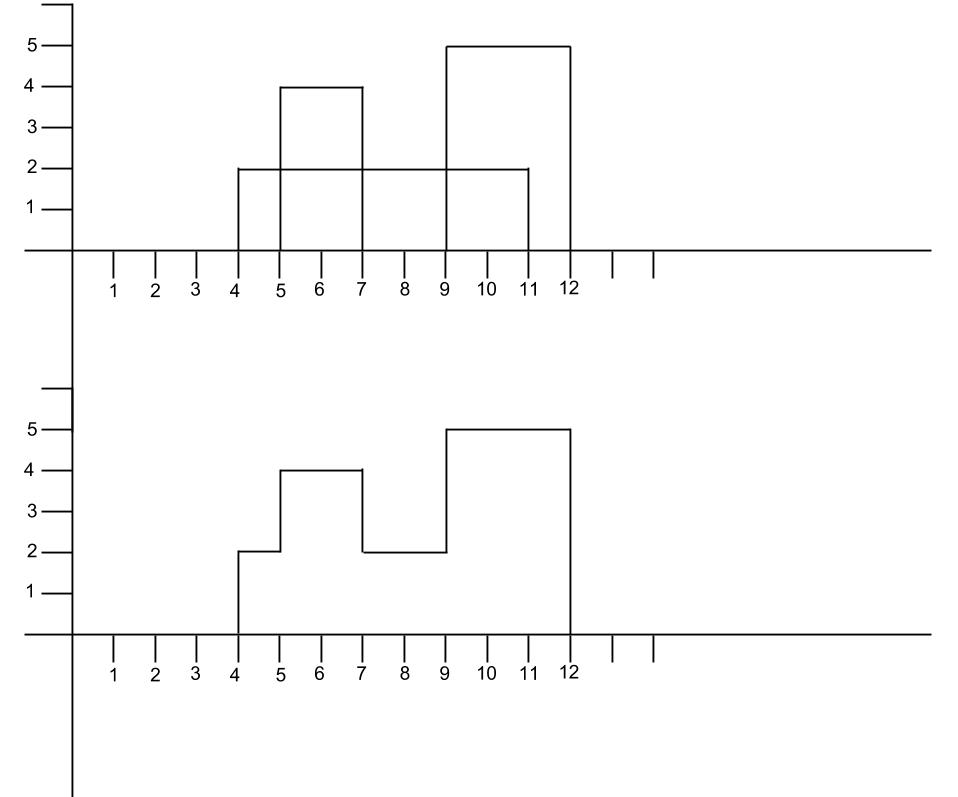
\includegraphics[scale=0.25]{imagenes/ej2.jpg}
  \end{center}
\end{figure}


\newpage


\subsection{Desarrollo de la idea y pseudocódigo.}

\vspace*{0.3cm}

El algoritmo propuesto para resolver este problema consiste en tomar a los edificios
por los 2 vértices que lo identifican (sus puntos con $Y \neq 0$).

Recorriendo esos vértices en orden, los pertenecientes a una pared izquierda
generarán un nuevo punto en el horizonte si son más altos que el último punto agregado
y los que correspondan a una pared derecha, si corresponden al final de la
altura actual, generarán un punto en la intersección con la siguiente altura mayor.

Para saber hasta dónde se debe bajar luego de un vértice de pared derecha, se
mantiene un multiconjunto de alturas. Cada vértice de pared izquierda carga su
altura y los de pared derecha la eliminan.

\begin{codebox}
\Procname{$\proc{calcularHorizonte}(vertices)$}
\li \Comment vertices: vector de vértices
\li $\id{horizonte} \gets \emptyset$
\li $\id{alturas} \gets \emptyset$
\li $\proc{sort}(vertices)$
\li $\id{vertice} \gets \proc{primero}(vertices)$
\li $\proc{agregar}(horizonte, <vertice.x, vertice.y>)$
\li $\proc{agregar}(alturas, vertice.y)$
\li \While $vertice \neq \proc{ultimo}(vertices)$
      \Do
\li     \If $vertice.posicion_{pared} \isequal izquierda$
          \Then
\li         \If $vertice_y > \proc{ultimo}(horizonte)_y$
              \Then
\li             \If $vertice_x > \proc{ultimo}(horizonte)_x$
                  \Then
\li                 $\proc{agregar}(horizonte, <vertice_x, vertice_y>)$
\li               \Else
\li                 $\proc{ultimo}(horizonte)_y \gets vertice_y$
                 \End
              \End
\li         $\proc{agregar}(alturas, vertice_y)$
\li       \Else
\li         $\proc{quitar}(alturas, vertice_y)$
\li         \If $vertice_y > \proc{maximo}(alturas)$
              \Then
\li             $\proc{agregar}(horizonte, <vertice_x, maximo(alturas)>)$
              \End
          \End
\li     $\id{vertice} \gets \proc{proximo}(vertice)$
      \End
\li \Return $\id{horizonte}$
\end{codebox}



\subsection{Justificación de la resolución y demostración de correctitud.}

\vspace*{0.3cm}


Dado un conjunto de edificios $E$, la solución será un conjunto de puntos
$S_E = \{p \in \mathbb{Z}^2 : \exists e \in E / (p_x = e_i \land p_y = e_y) \land
p \notin T_E\} \cup \{p \in \mathbb{Z}^2 : \exists e \in E / (p_x = e_d \land p
\notin T_E) \land p_y = \max({\{e_y : e \in E \land e_i \leq p_x < e_d\} \cup \{0\}})\}$,
donde $T_E = \{p \in \mathbb{Z}^2 : \exists e \in E / (e_i \leq p_x \leq e_d \land p_y \leq e_y)\}$
son los puntos cubiertos por todos los edificios.

Para demostrar la correctitud de este algoritmo, veremos que cumple con la
definición dada más arriba.

Primero, el algoritmo ordena y recorre en orden todos los puntos de los edificios.

Por cada punto $p$, se revisa si corresponde agregar o modificar un punto a la
solución parcial, de la siguiente manera:

\begin{itemize}
  \item Si es un vértice izquierdo del edificio, $p = <e_i, e_y>$, se carga su
  altura en el multiconjunto de alturas.
  \begin{itemize}
    \item Si su altura es menor o igual a la del último punto cargado, como
    vamos recorriendo en orden, podemos asegurar que $\exists e \in E / e_i \leq p_x \leq e_d \land p_y \leq e_y$,
    por lo tanto está cubierto por un edificio y no corresponde cargarlo.

    \item Si su altura es mayor a la del último punto y también su coordenada $X$,
    entonces podemos asegurar que $\nexists e \in E / e_i < p_x \land p_y \leq e_y$,
    es decir, no está cubierto por un edificio que comience antes, entonces cargamos
    el punto. Pero:

    \item Si su altura es mayor a la del último punto y sus coordenadas $X$ son
    iguales, quiere decir que el punto cargado no estaba cubierto por uno que comience
    antes, sino por uno que comienza en el mismo punto, pero que es más alto.
    En este caso reemplazamos la atura cargada en el último punto, por la altura
    de este.
  \end{itemize}

  \item Si es un vértice derecho del edificio, $p = <e_d, e_y>$, se elimina su
  altura del munticonjunto.
  \begin{itemize}
    \item Si su altura sigue siendo igual a la máxima del multiconjunto, podemos
    afirmar que $\exists e \in E / e_i \leq p_x \leq e_d \land p_y \leq e_y$ y
    no corresponde cargar un nuevo punto.

    \item Si su altura es mayor a la máxima del multiconjunto,
    $\nexists e \in E / e_i < p_x \land p_y \leq e_y$, por lo tanto marca el
    final de un edificio en el horizonte. Y se carga el punto $p' = <e_d, \max(alturas)>$,
    ya que al recorrer en orden, en alturas quedan $\{e_y \in \mathbb{Z} : e \in E / e_i \leq p_x < e_x\}$
  \end{itemize}
\end{itemize}

De esta forma, nos aseguramos de considerar todos los puntos posibles y terminando
únicamente con los que corresponden.


\subsection{Análisis de complejidad.}

\vspace*{0.3cm}

Respecto de las operaciones utilizadas de \verb|vector|, \verb|size| $\in O(1)$,
\verb|back| $\in O(1)$, \verb|resize| $\in O(n)$, \verb|push_back| $\in O(1)$,
\verb|begin| $\in O(1)$, \verb|end| $\in O(1)$ y \verb|operator[]| $\in O(1)$.

\noindent
En \verb|Vertice|, el constructor y el \verb|operator<| son $O(1)$. También
tiene complejidad constante el constructor de \verb|Punto|.

\noindent
En las operaciones utilizadas de \verb|multiset|, \verb|insert| $\in O(\log n)$,
\verb|erase| $\in O(1)$, \verb|find| $\in O(\log n)$, \verb|empty| $\in O(1)$ y
\verb|rbegin| $\in O(1)$.

\noindent
Sobre los iteradores, se realizan las operaciones \verb|++| y \verb|*|, ambas
con complejidad constante.

\noindent
Se implementó la función \verb|maximo|, que dado un \verb|multiset|, devuelve
el mayor de sus elementos, o 0 si el \verb|multiset| está vacío. Dicha función
tiene complejidad constante, pues \verb|empty| $\in O(1)$ y \verb|rbegin| $\in O(1)$.

\noindent
El algoritmo \verb|sort| utilizado tiene complejidad $O(n \log n)$.

\noindent

\begin{enumerate}
  \item Se iteran todos los edificios y se cargan sus 2 vértices, dentro
  del ciclo la asignación es constante. Por lo tanto el ciclo $\in O(n)$

  \item Se ordenan los vértices con \verb|sort|, con la función de comparación
  constante. Este paso se realiza en $O(n)$

  \item Se itera sobre cada vértice y en cada iteración se realizan una cantidad
  constante de comparaciones, asignaciones, todas $\in O(1)$. Y hasta una operación
  (\verb|agregar| o \verb|quitar|) $\in O(\log n)$.

  \item Al tener $2n$ vértices, la complejidad total del ciclo $\in O(n \log n)$.

  \item La complejidad total es la suma de estos pasos: $O(n \log n)$
\end{enumerate}


\newpage


\subsection{Experimentación y gráficos.}

\vspace*{0.3cm}

\subsubsection{Test 1 - benchmark caso aleatorio}

En este test, $n$ (cantidad de edificios) se inicializa en 100 y va incrementándose también de a 100, 
hasta alcanzar 100000. Las coordenadas de los vértices se genera aleatoriamente, de forma uniforme.
 
Para cada instancia, se toma el \textbf{valor mínimo} de cantidad de ciclos luego de \textbf{25 corridas}. 

\vspace*{0.5cm}

\begin{figure}[h]
  \begin{center}
    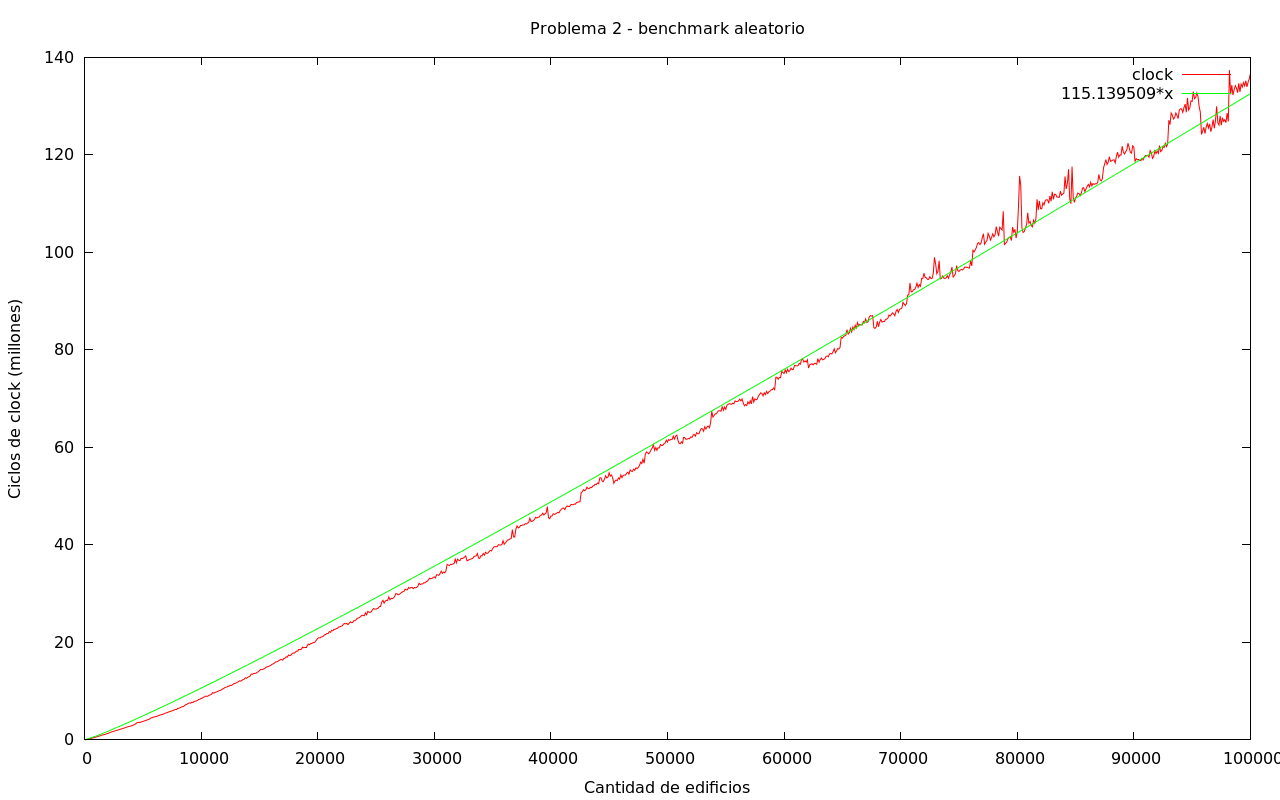
\includegraphics[scale=0.35]{imagenes/grafico-2.png}
  \end{center}
\end{figure}

\vspace*{0.5cm}

En este gráfico podemos apreciar que, los valores que toma la curva que representa la cantidad de ciclos 
de clock empieza tomando valores menores a nuestra curva de referencia, para después acercarse bastante y 
luego superarla, tal como se comportaría una curva del estilo $y = x*log x$, pero en este caso está más 
"linealizada" por tratarse del caso aleatorio.

\newpage


\subsubsection{Test 2 - benchmark del peor caso}

En este test, $n$ (cantidad de edificios) se inicializa en 100 y va incrementándose también de a 100, 
hasta alcanzar 100000. Tomamos como peor caso, una instancia en la cual se generan alturas de 1 a $n$, 
se mezclan y luego se generan paredes que van "achicándose", es decir, para la primer altura tenemos 
\verb|1 2n|, para la segunda \verb|2 2n-1| y así sucesivamente.
 
Para cada instancia, se toma el \textbf{valor mínimo} de cantidad de ciclos luego de \textbf{25 corridas}.

\vspace*{0.5cm}

\begin{figure}[h]
  \begin{center}
    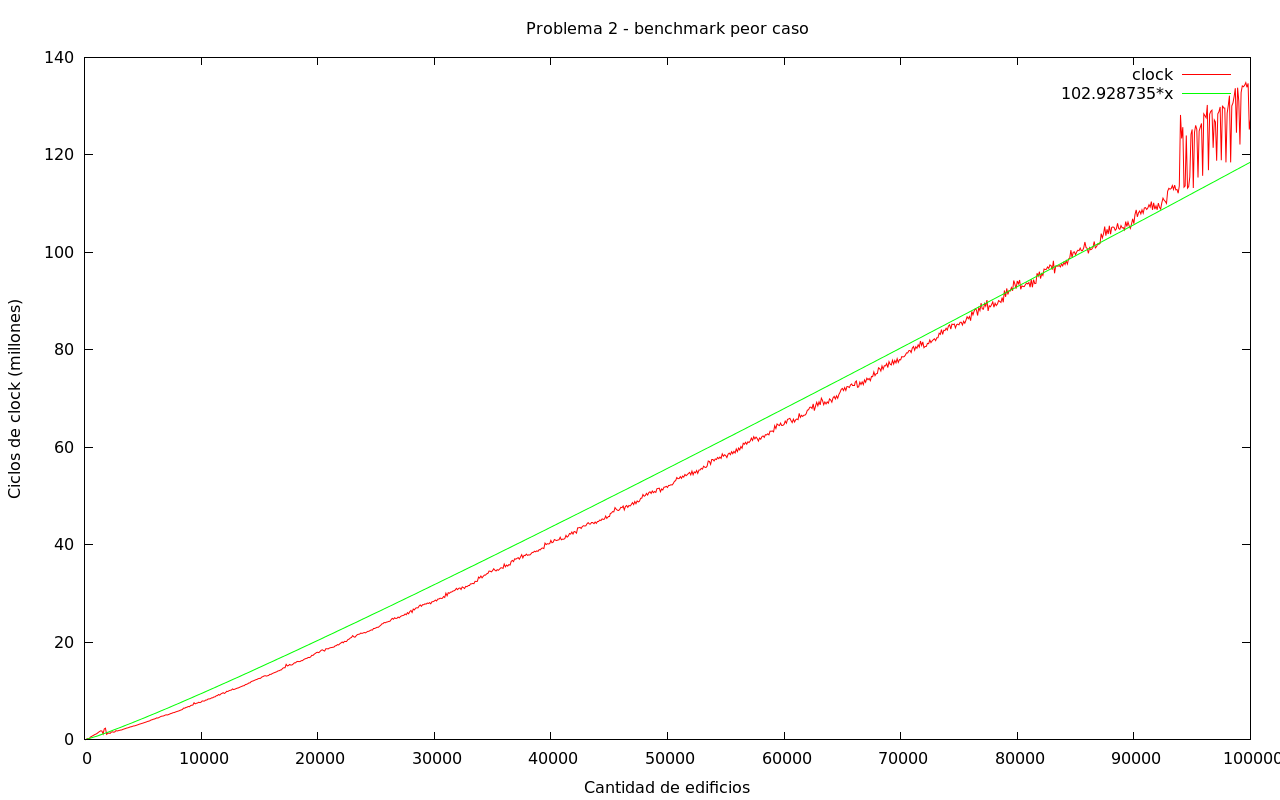
\includegraphics[scale=0.35]{imagenes/grafico-2-peor.png}
  \end{center}
\end{figure}

\vspace*{0.5cm}

En este gráfico podemos apreciar que, al igual que en el experimento aleatorio, los valores que toma la curva 
que representa la cantidad de ciclos de clock empieza tomando valores menores a nuestra curva de referencia, 
para después acercarse bastante y luego superarla, tal como se comportaría una curva del estilo $y = x*log x$, 
pero, a diferencia del anterior, en el punto donde la curva de referencia es superada, la curva que mide nuestro 
algoritmo crece a mayor velocidad (para $n$ = 90000 aproximadamente, la curva de referencia ya se ve superada, 
mientras que en el experimento aleatorio se mantenían similares).


\newpage


\subsubsection{Test 3 - benchmark del mejor caso}

En este test, $n$ (cantidad de edificios) se inicializa en 100 y va incrementándose también de a 100, 
hasta alcanzar 100000. Tomamos como mejor caso una instancia con un gran edificio, que posee dentro 
edificios disjuntos (es decir, cuyas paredes no se instersectan).

Para cada instancia, se toma el \textbf{valor mínimo} de cantidad de ciclos luego de \textbf{25 corridas}.


\begin{figure}[h]
  \begin{center}
    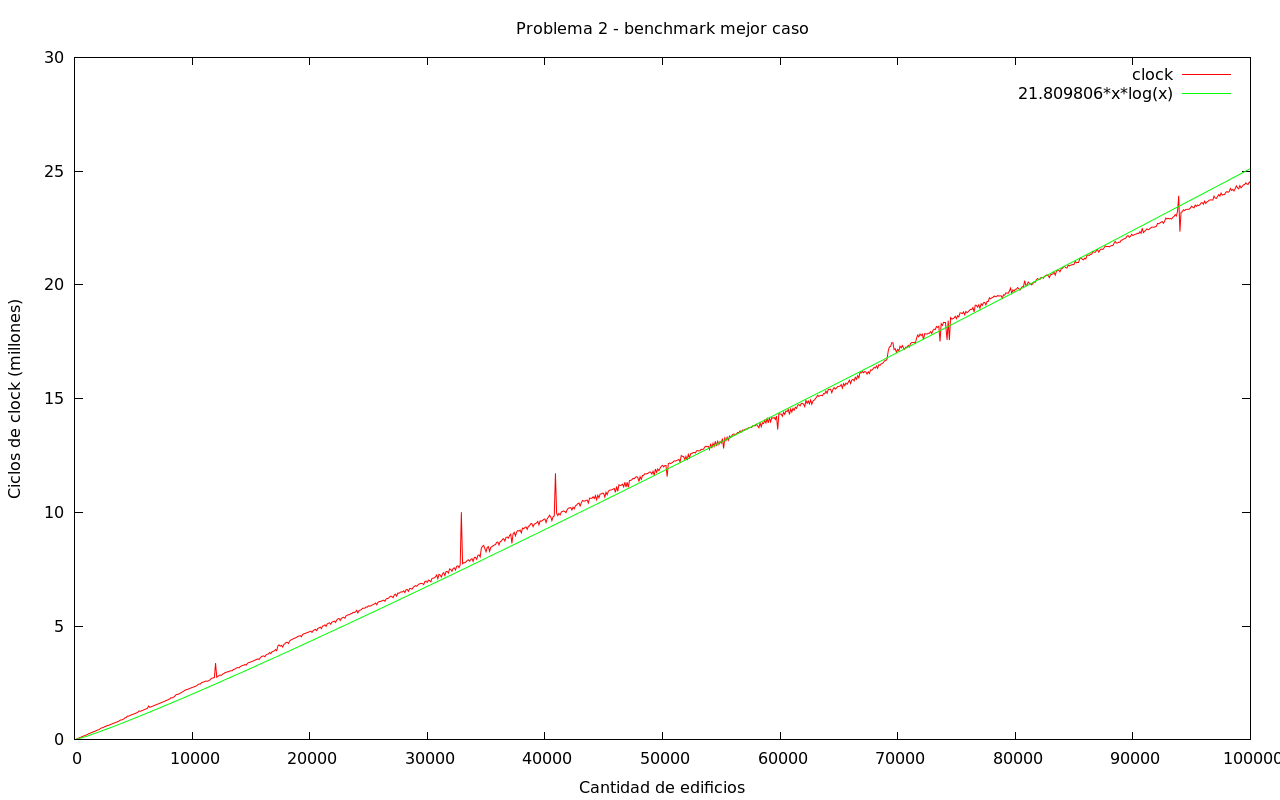
\includegraphics[scale=0.35]{imagenes/grafico-2-mejor.png}
  \end{center}
\end{figure}


En este gráfico podemos apreciar que, a diferencia de los dos experimentos anteriores, el comportamiento 
del algoritmo es prácticamente lineal, reduciendo además la cantidad de ciclos requeridos en un 75\% 
aproximadamente. También es importante notar que la curva que representa los valores en ciclos requeridos 
por nuestro algoritmo se mantiene acotada superiormente por la curva tomada de referencia. Entendemos que 
para aquellos puntos donde sí la supera, se deben más bien a errores en la medición o momentos de sobrecarga 
del procesador. 
